\documentclass[11pt]{beamer}
\usepackage[utf8]{inputenc}
\usepackage[T1]{fontenc}
\usepackage{lmodern}
\usepackage{amsmath}
\usepackage{amsfonts}
\usepackage{amssymb}
\usepackage{graphicx}
\usetheme{Boadilla}
\usepackage{media9}
\usepackage{multimedia}
\usepackage{pdfpages}
\usepackage{hyperref}
\usepackage[labelformat=empty]{caption}

\begin{document}
	\author{Julien Nyambal}
	\title{Why GPUs for Machine Learning?}
	%\subtitle{}
	\logo{entelect}
	\institute{Entelect}
	\logo{
\includegraphics[height=0.5cm]{entelect.png}}
	%\date{}
	\setbeamertemplate{navigation symbols}{}
	\begin{frame}[plain]
		\maketitle
	\end{frame}

\begin{frame}
	\centering
	The CPU is the heart of the computer, and the GPU his soul ...
\end{frame}

	\begin{frame}
		\frametitle{What will be covered ...}
		\tableofcontents
	\end{frame}

\section{What is Machine Leaning?}
\begin{frame}
	\frametitle{What is Machine Leaning?}
	\begin{figure}
		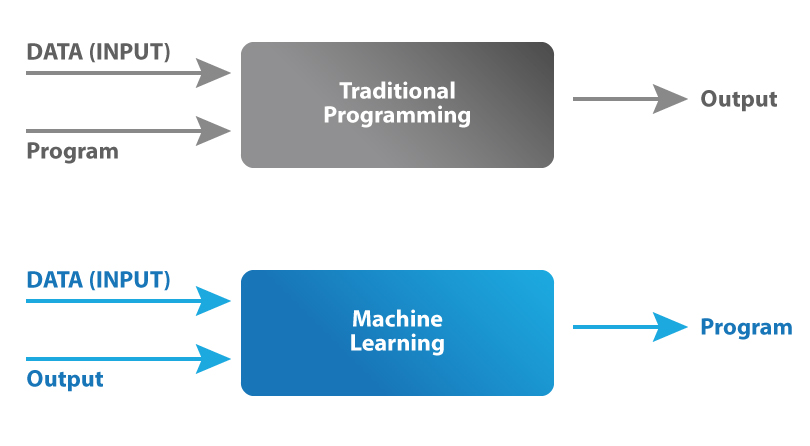
\includegraphics[width=100mm,scale=0.7]{ml}
		\caption{A general definition of a ML}
	\end{figure}
\end{frame}

\begin{frame}
	\frametitle{What is Machine Leaning?: Conceptual Overview}
	\begin{figure}
	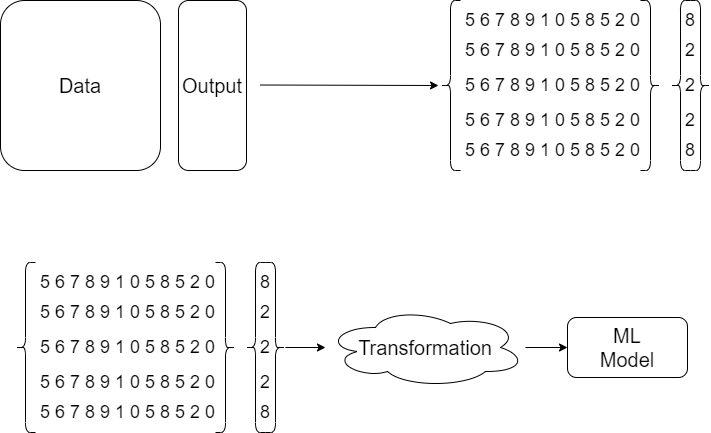
\includegraphics[width=100mm,scale=0.7]{ml_concept}
	\caption{ML - Conceptual}
\end{figure}
\end{frame}

\begin{frame}
	\frametitle{What is Machine Leaning?: Deep Learning}
\begin{figure}
	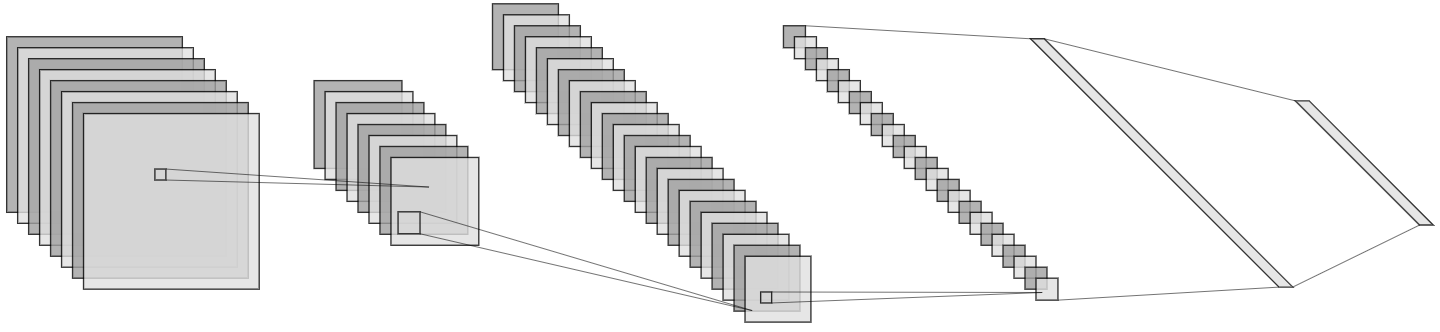
\includegraphics[width=55mm,scale=0.5]{cnn}\hspace{2mm}
	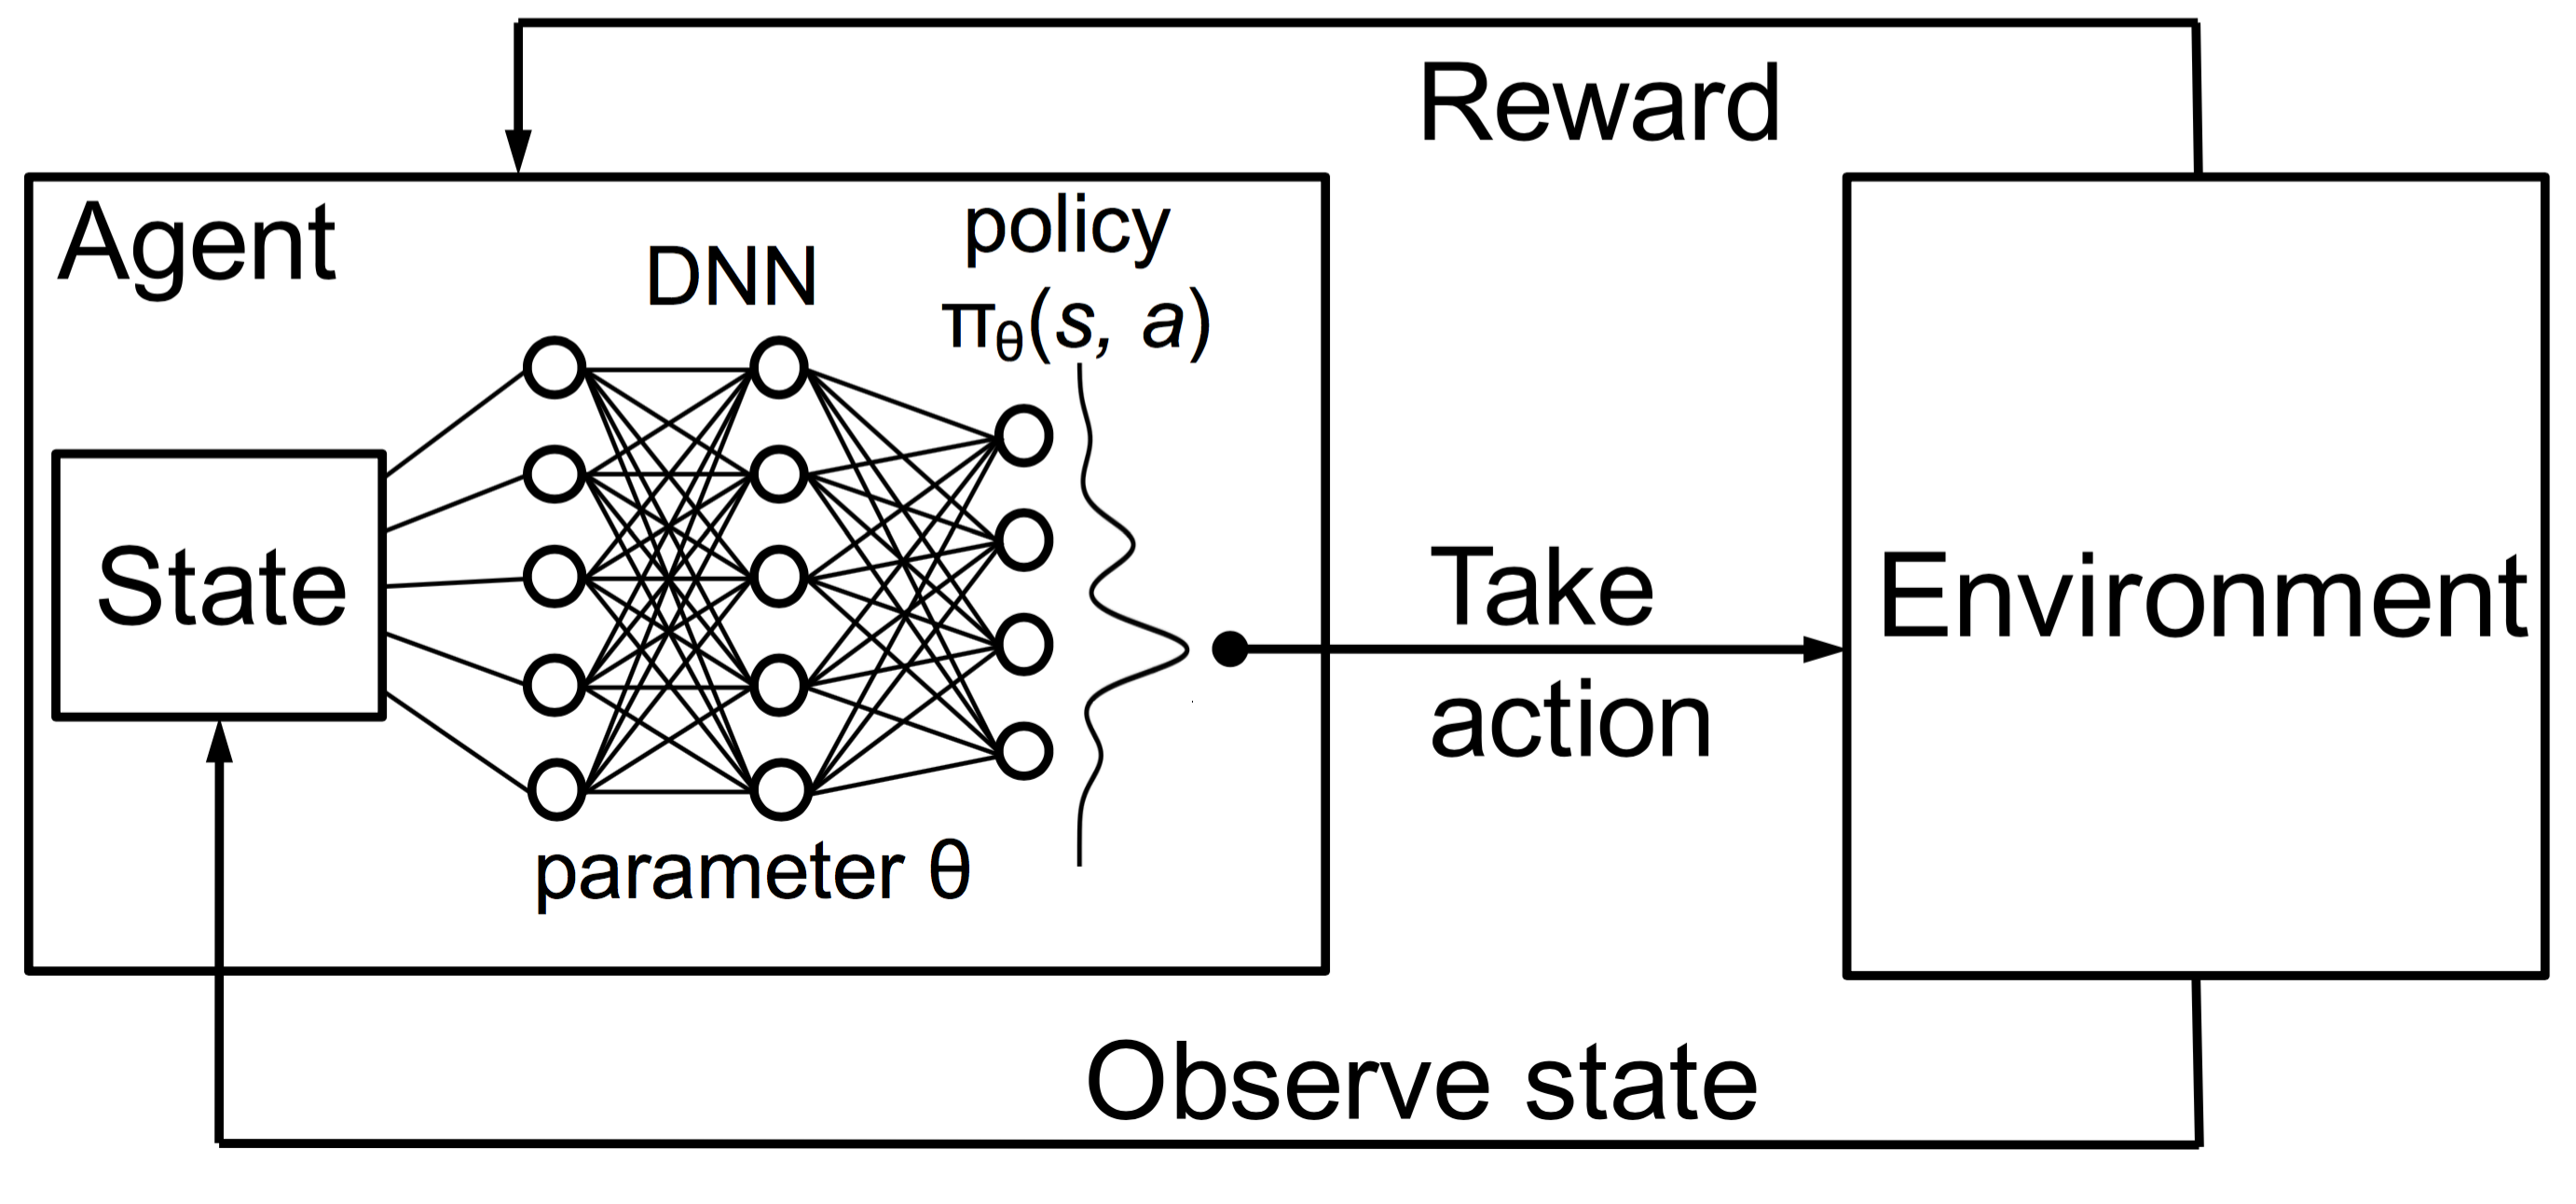
\includegraphics[width=55mm,scale=0.5]{drl}
	\\[\smallskipamount]
	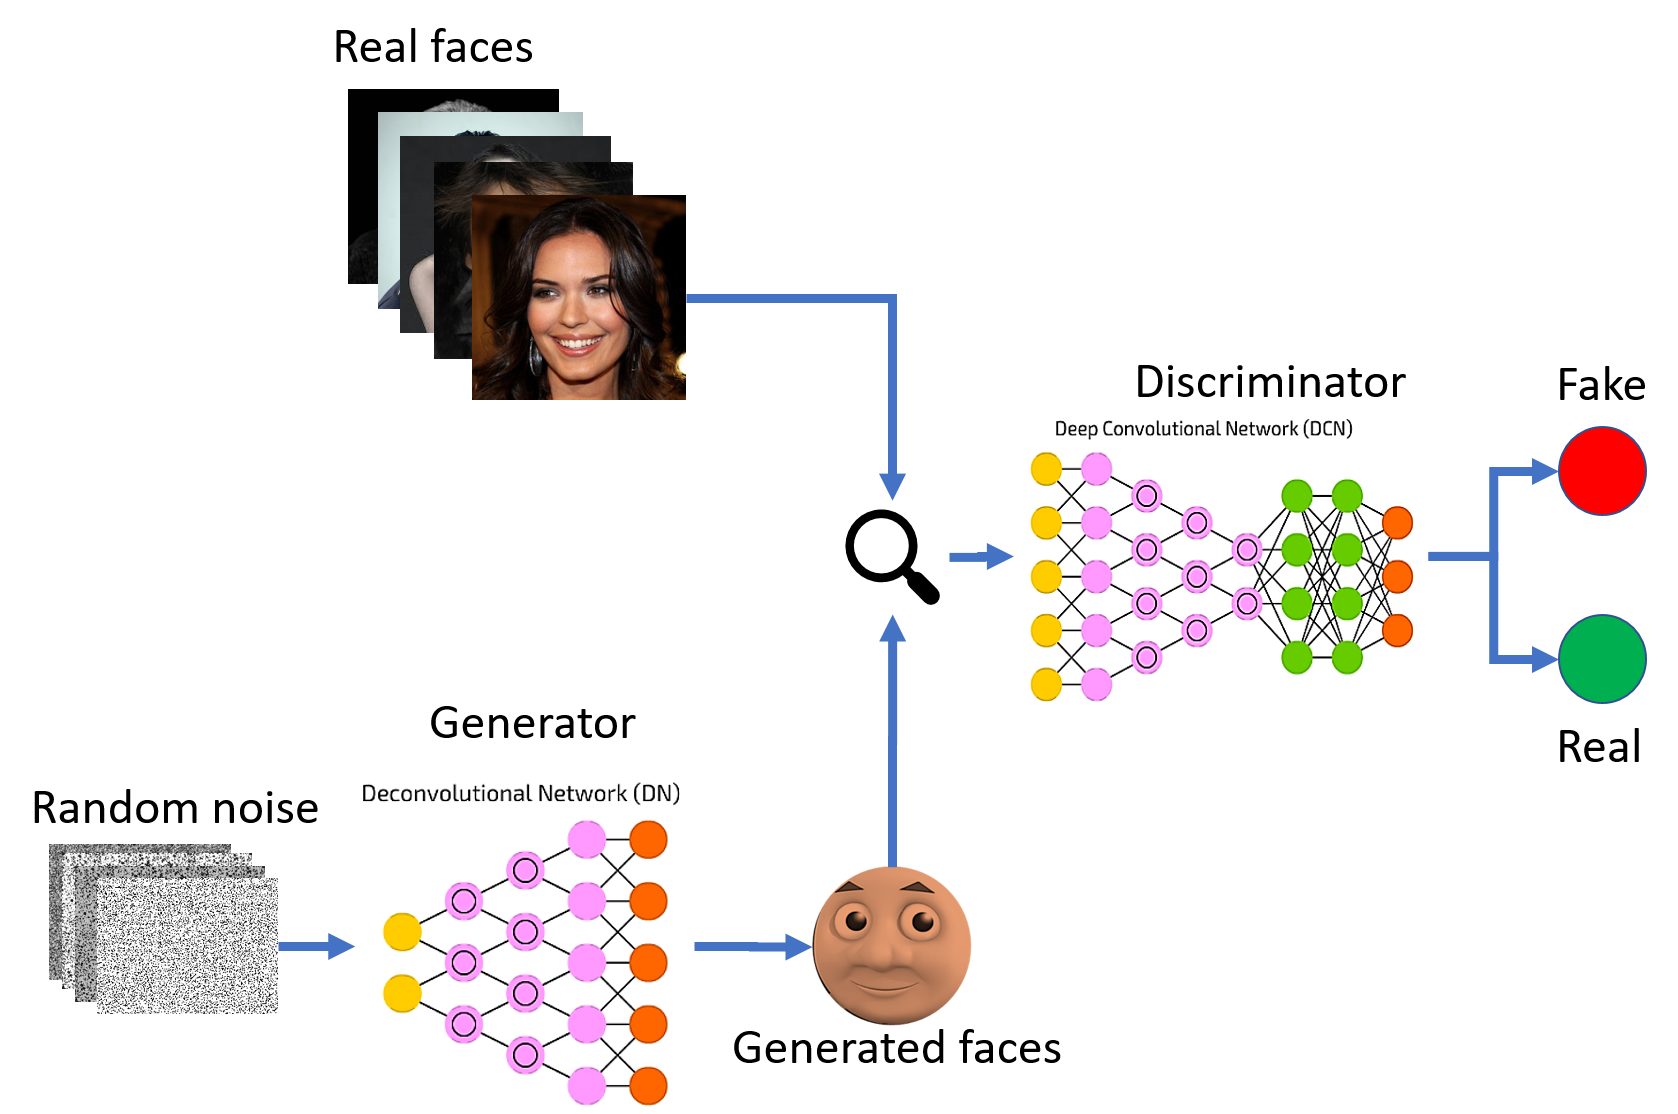
\includegraphics[width=55mm,scale=0.5]{gan}\hspace{2mm}
	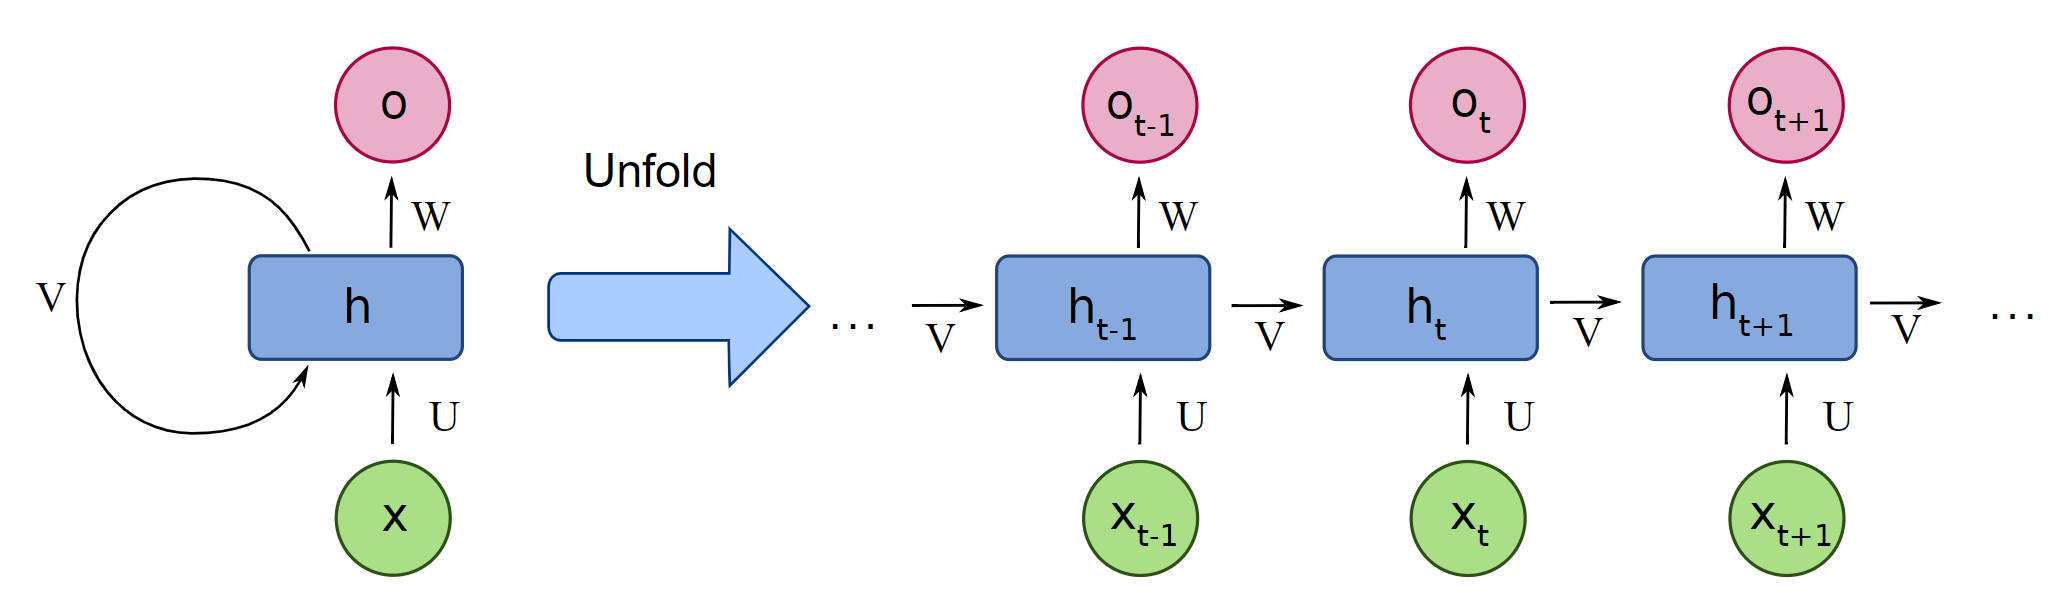
\includegraphics[width=55mm,scale=0.5]{rnn}
\end{figure}
\end{frame}

\section{Tensors: A naive description}
\begin{frame}
	\frametitle{Tensors: A naive description}
		\begin{figure}
		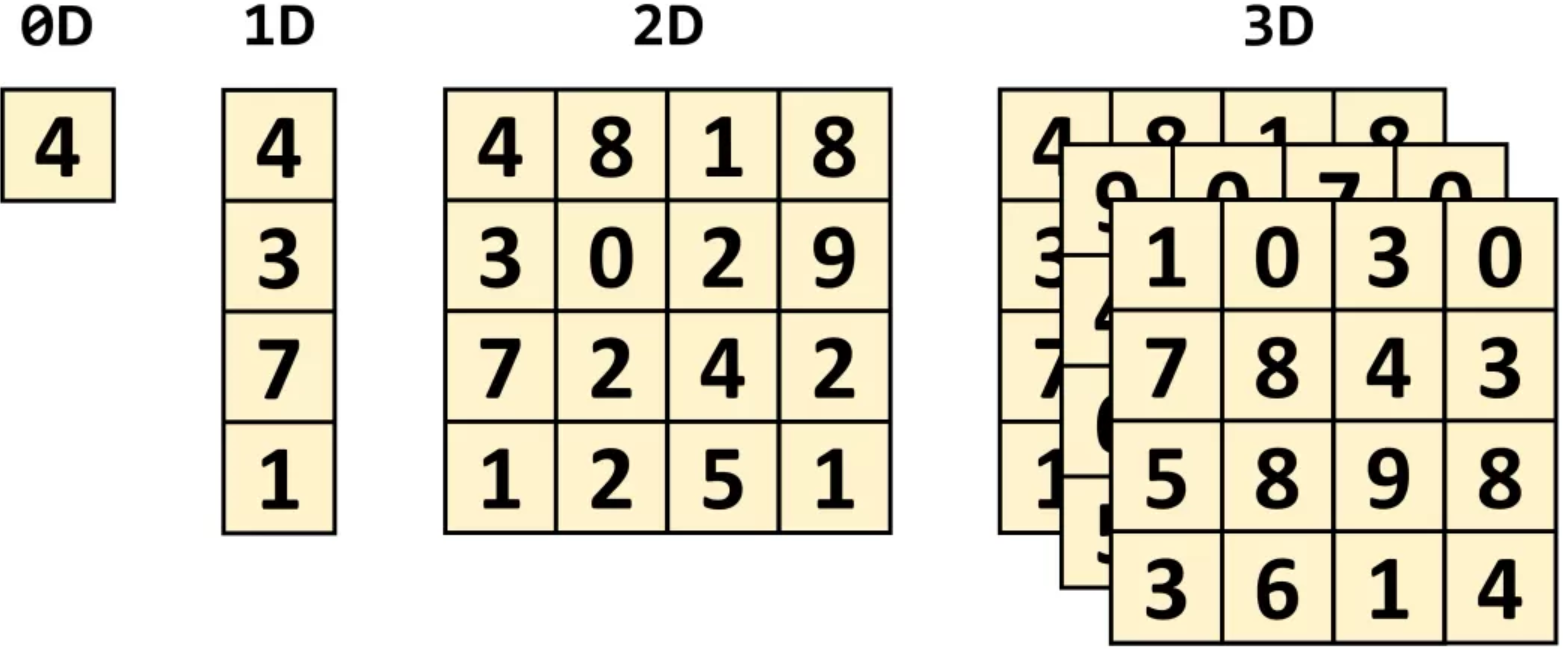
\includegraphics[width=100mm,scale=0.7]{tensors}
		\caption{A general definition of a Tensor}
	\end{figure}
\end{frame}

\begin{frame}
	\frametitle{Tensors: Operations - Addition}
	\subsection{Addition}
		 \begin{figure}
		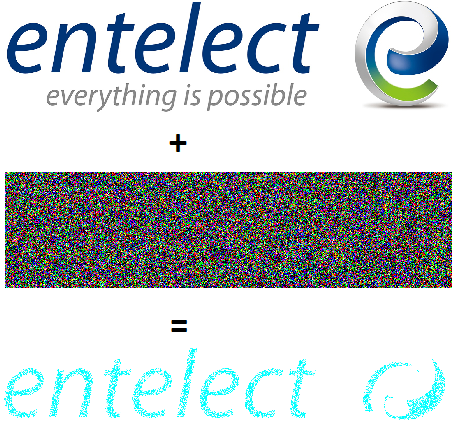
\includegraphics[width=50mm,scale=0.7]{add_noise}
	\end{figure}
\end{frame}

\begin{frame}
	\frametitle{Tensors: Operations - Matrix Multiplication}
	\subsection{Matrix Multiplication}
\begin{itemize}
	\item The most used operation in Machine Learning/Deep Learning
	\item There are many types of Matrix Multiplication of \textit{\textbf{MatMul}}. There 3 are the most common matrix multiplication:
	\begin{itemize}
		\item Brute Force Multiplication
		\item Column-Wise Multiplication
		\item Block Multiplication		
	\end{itemize}
\end{itemize}
\end{frame}

\begin{frame}
	\frametitle{Tensors: Operations - Matrix Multiplication}
	
	\begin{figure}
		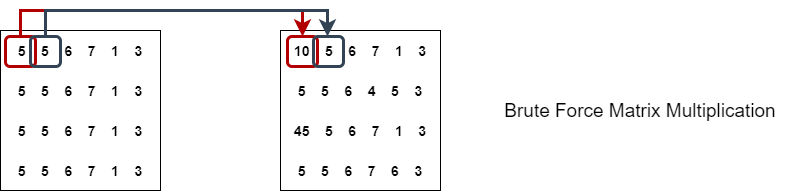
\includegraphics[width=100mm,scale=0.5]{brute_force_mat_mul}
		\\[\smallskipamount]
		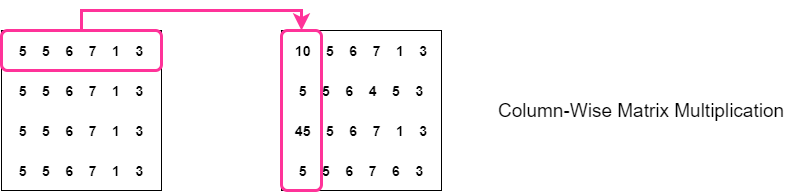
\includegraphics[width=100mm,scale=0.5]{column_wise_mat_mul}
		\\[\smallskipamount]
		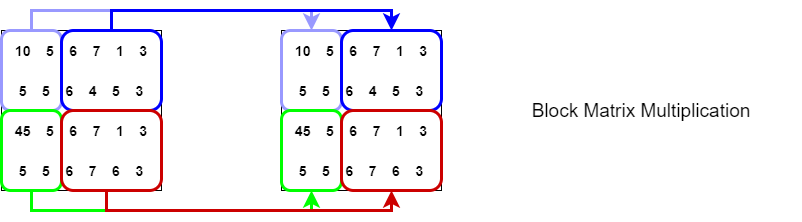
\includegraphics[width=100mm,scale=0.5]{block_multiplication}
	\end{figure}
	
%			\begin{figure}
%				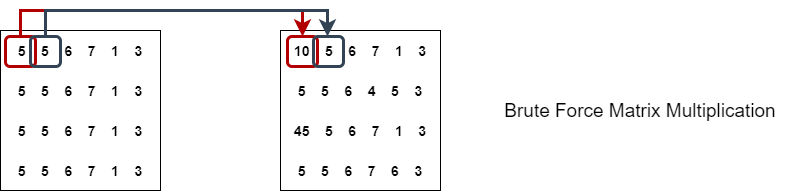
\includegraphics[width=50mm,scale=0.5]{brute_force_mat_mul}
%			\end{figure}
%
%			\begin{figure}
%				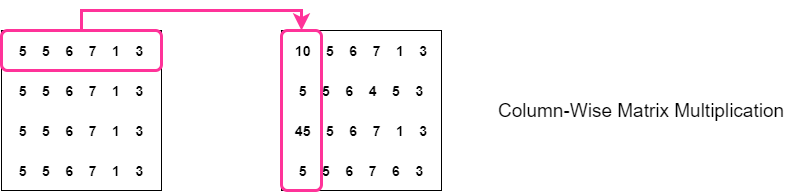
\includegraphics[width=50mm,scale=0.5]{column_wise_mat_mul}
%			\end{figure}
%
%			\begin{figure}
%				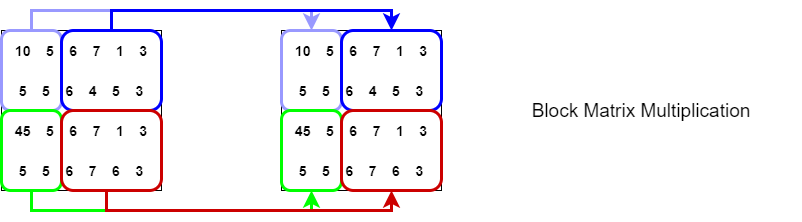
\includegraphics[width=40mm,scale=0.5]{block_multiplication}
%			\end{figure}
\end{frame}

\begin{frame}
	\frametitle{Tensors: Operations - Matrix Multiplication}
	\centering
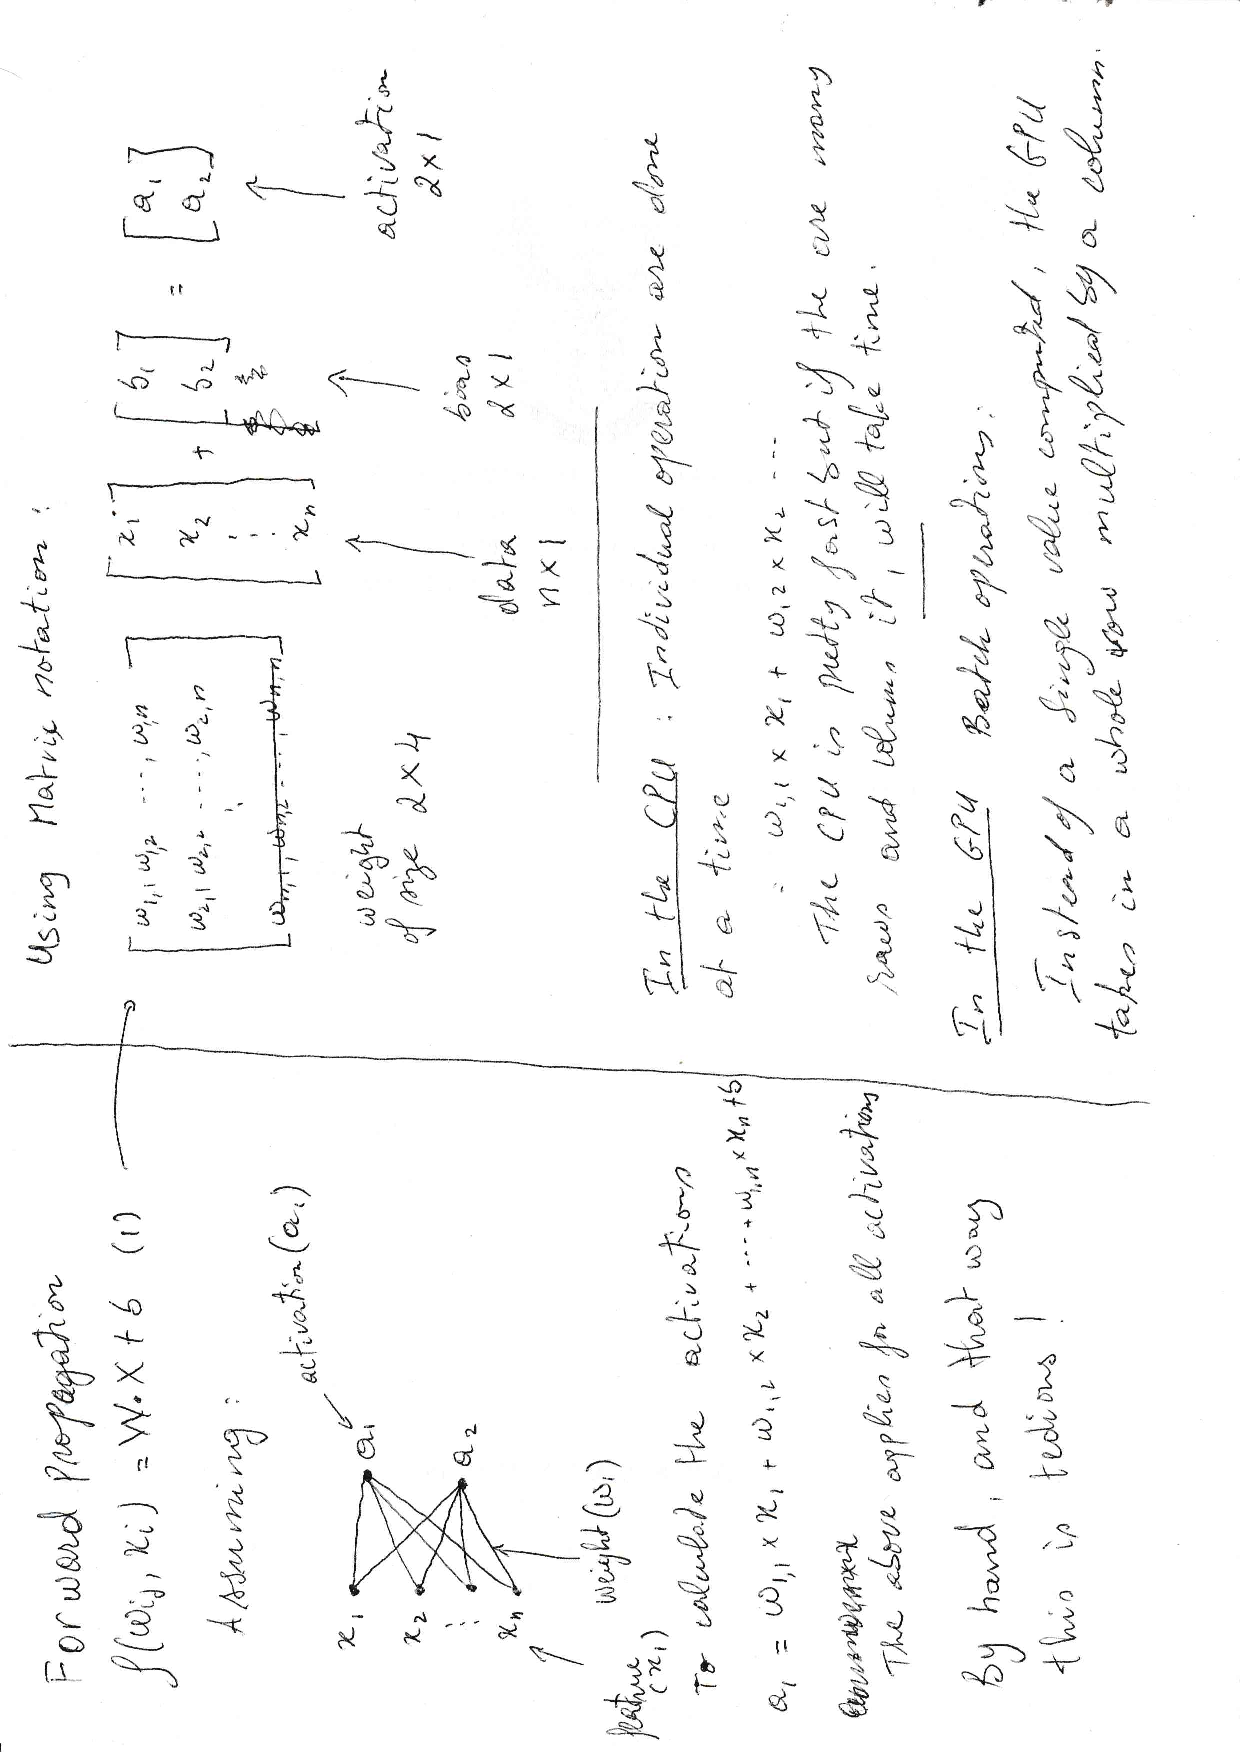
\includegraphics[width=\textwidth+2cm,height=\textheight+2cm,keepaspectratio, angle = -90 ]{demo.pdf}
\end{frame}

\section{Tensor Operations on Hardware}
\begin{frame}{movie}
	\frametitle{Matrix Computation on GPU vs CPU}
	\subsection{Matrix Computation on GPU vs CPU}
	\begin{figure}[h!]
	\centering
	{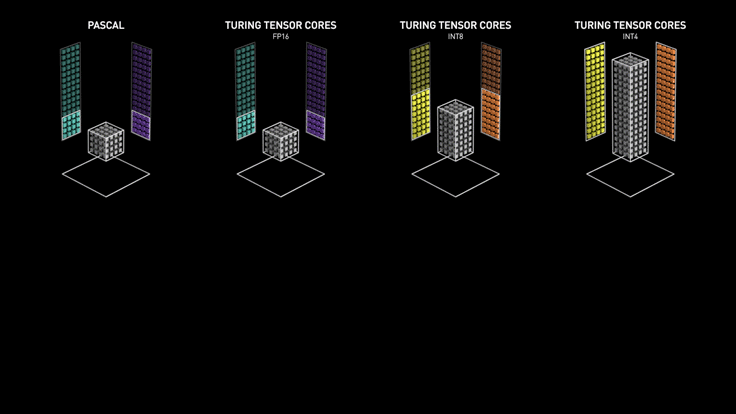
\includegraphics[width=1.0\textwidth]{gpugif.png}}
	\end{figure}
\end{frame}

\section{RAM, CPU, GPU, TPU}

\begin{frame}
	\frametitle{RAM, GPU, CPU, TPU}
	\subsection{TPU: Tensor Processing Unit}
\begin{figure}
	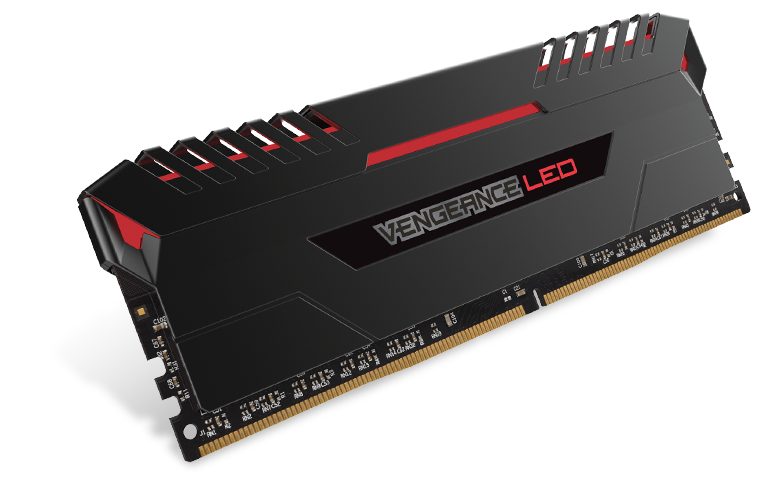
\includegraphics[width=50mm,scale=0.5]{ram5}\hspace{2mm}
	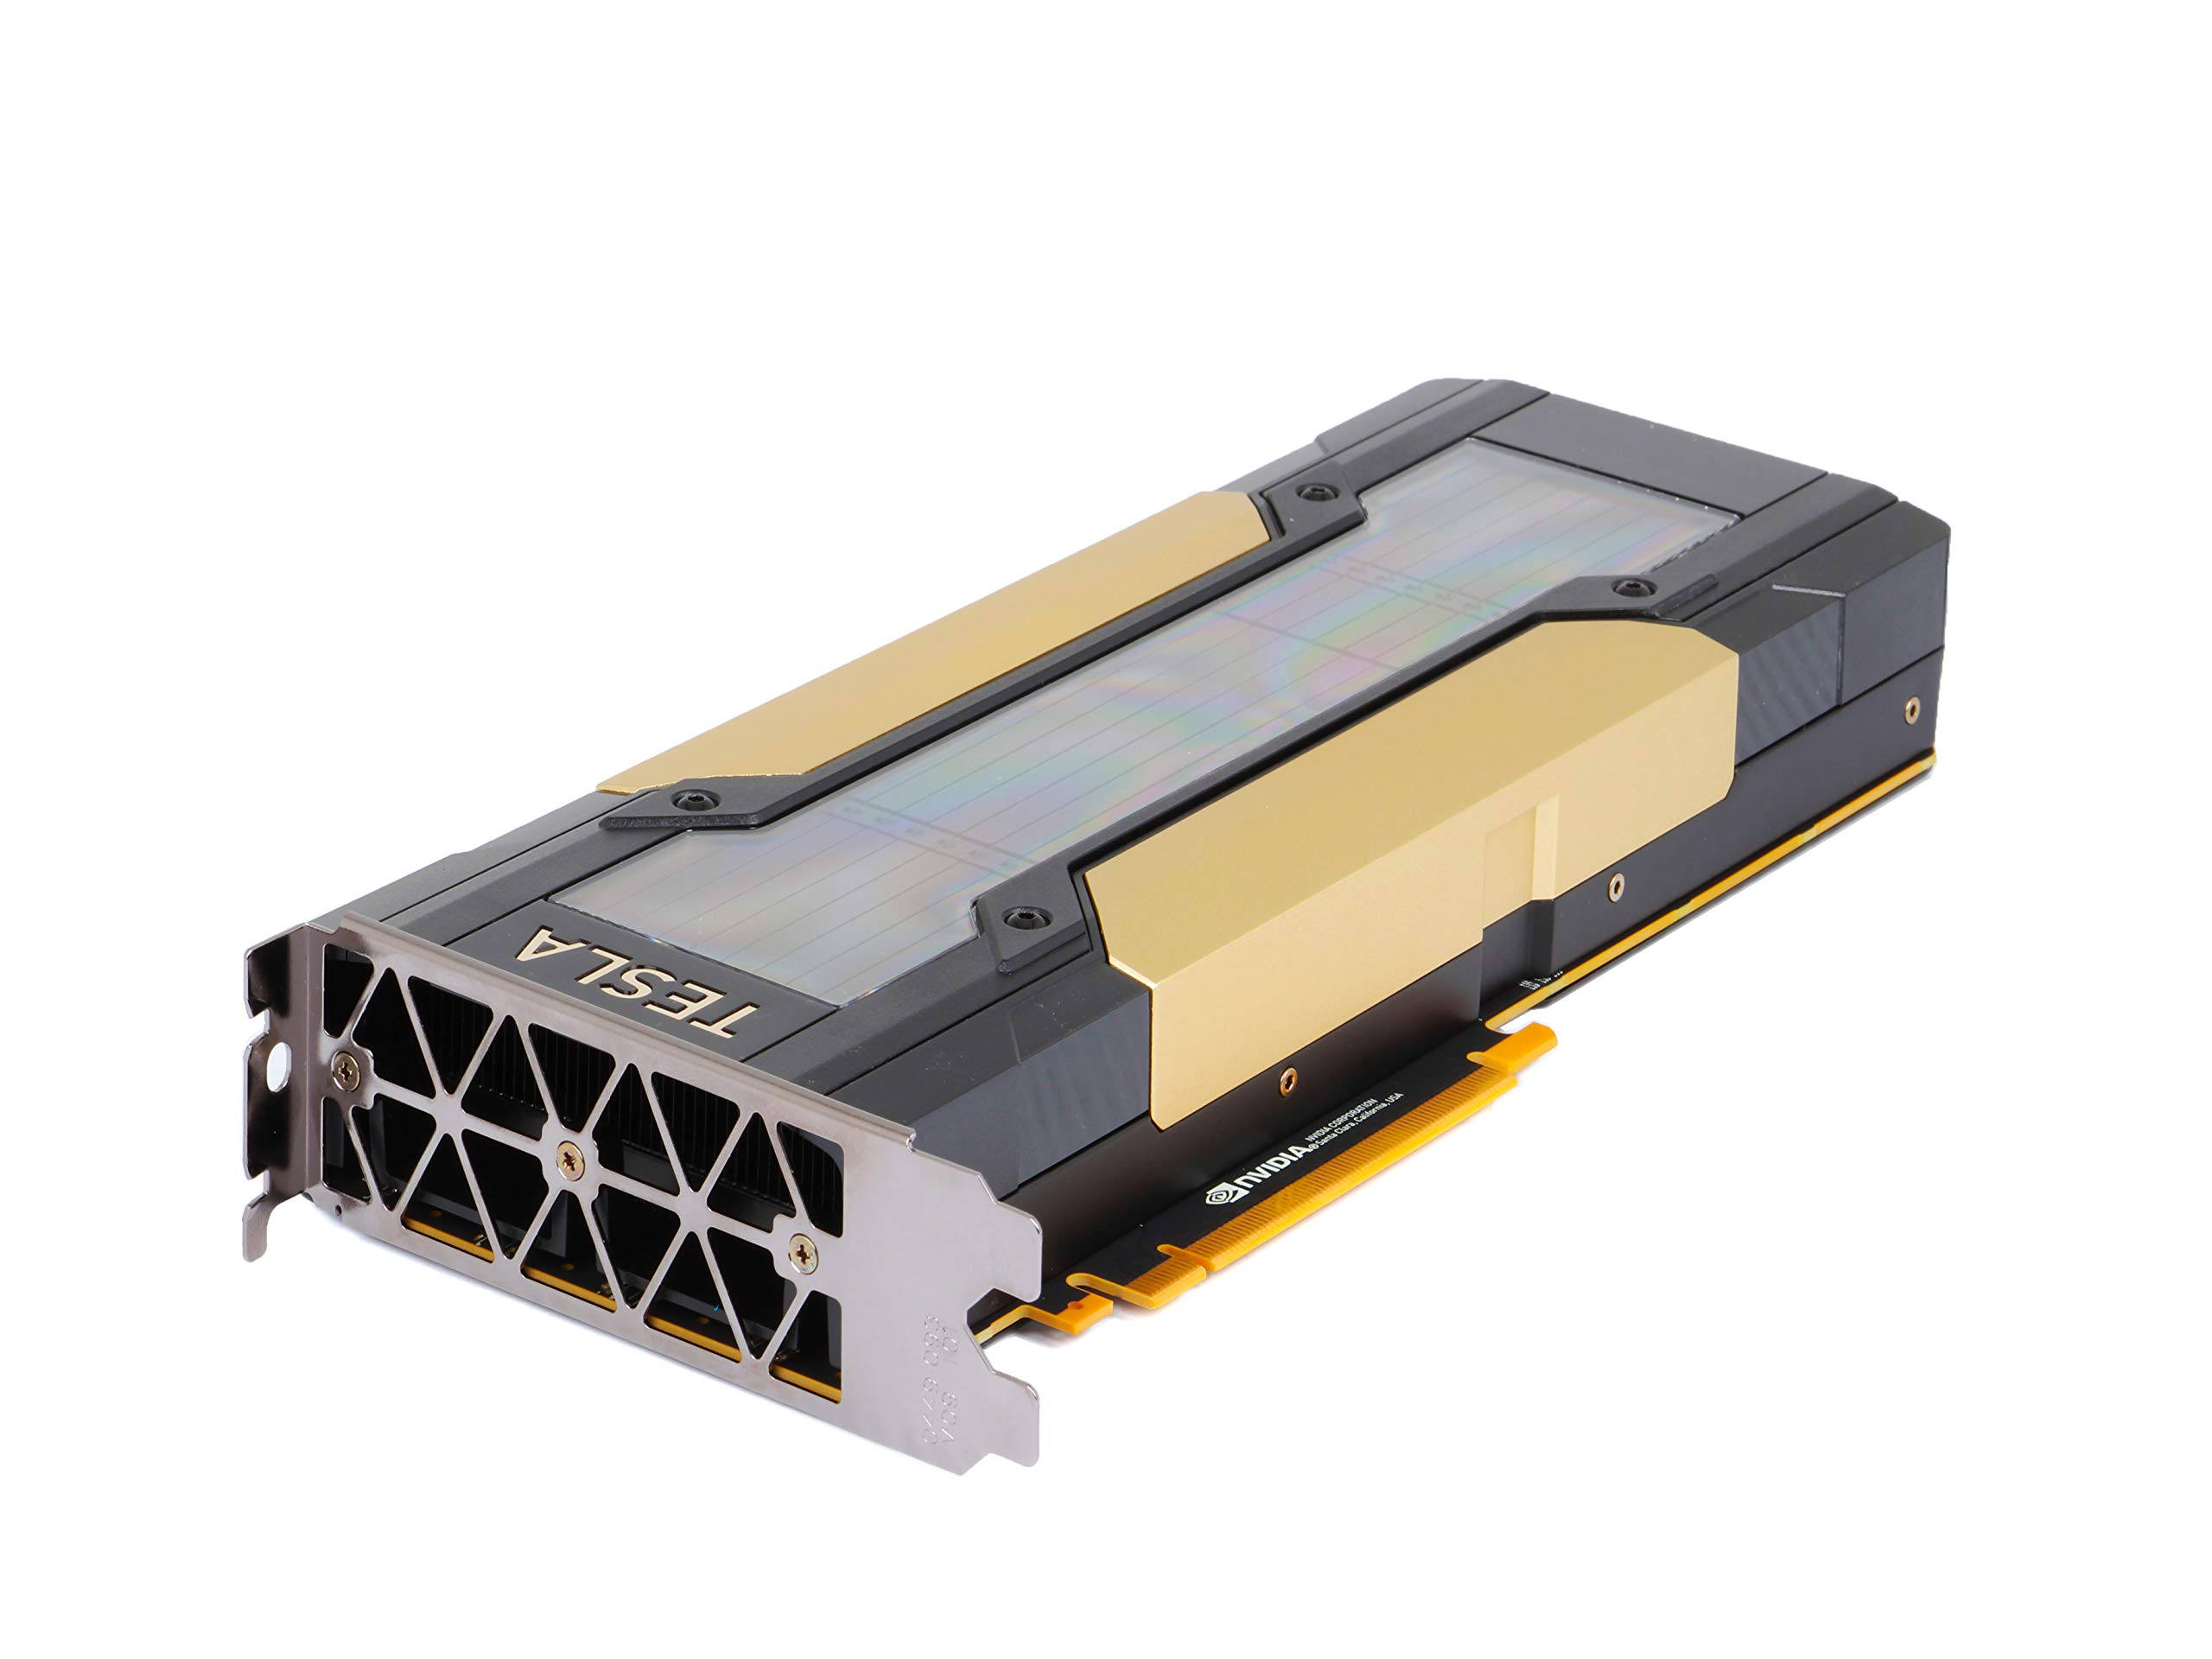
\includegraphics[width=50mm,scale=0.5]{v100}
	\\[\smallskipamount]
	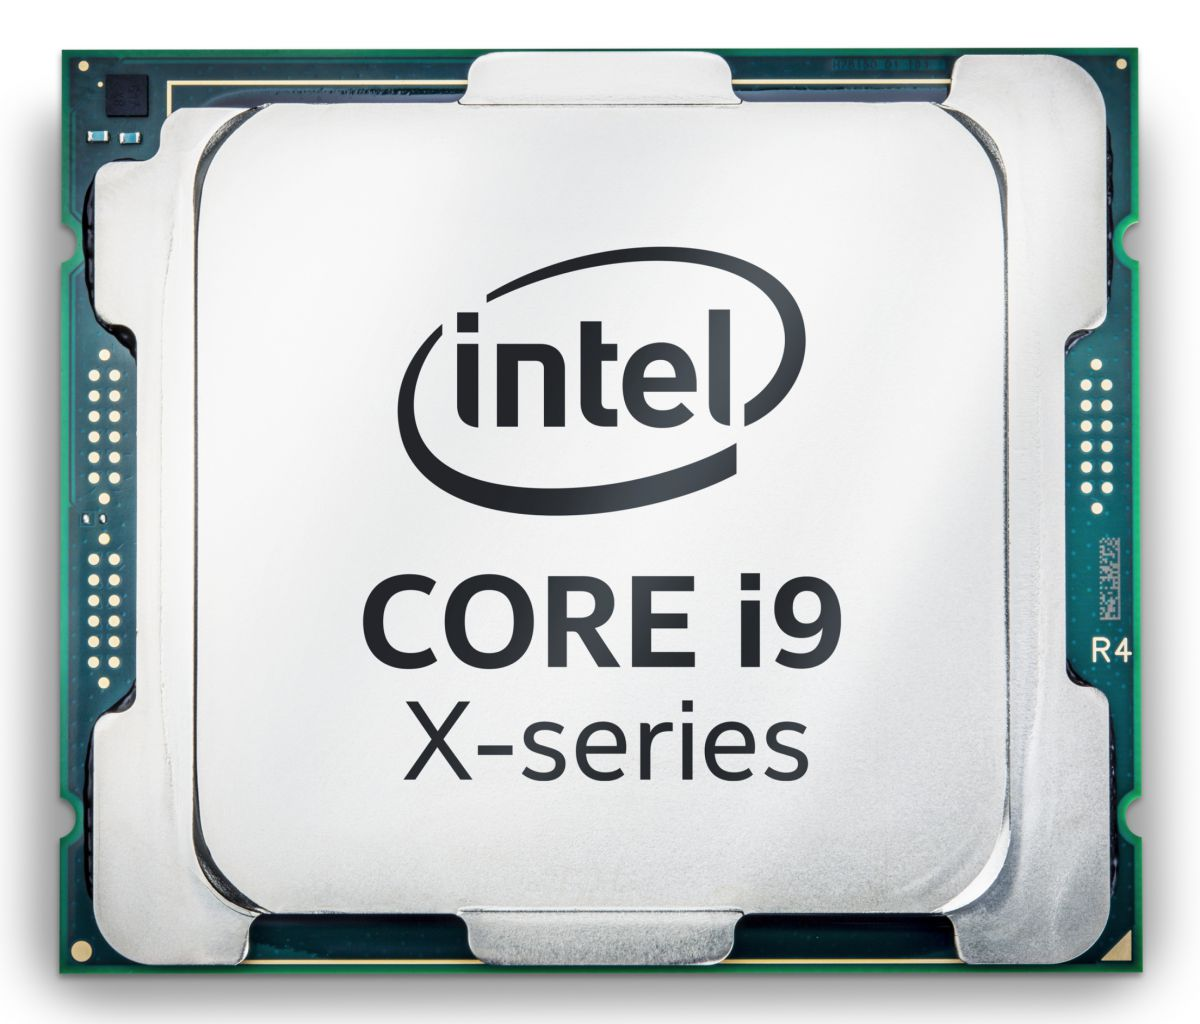
\includegraphics[width=50mm,scale=0.5]{cpu2}\hspace{2mm}
	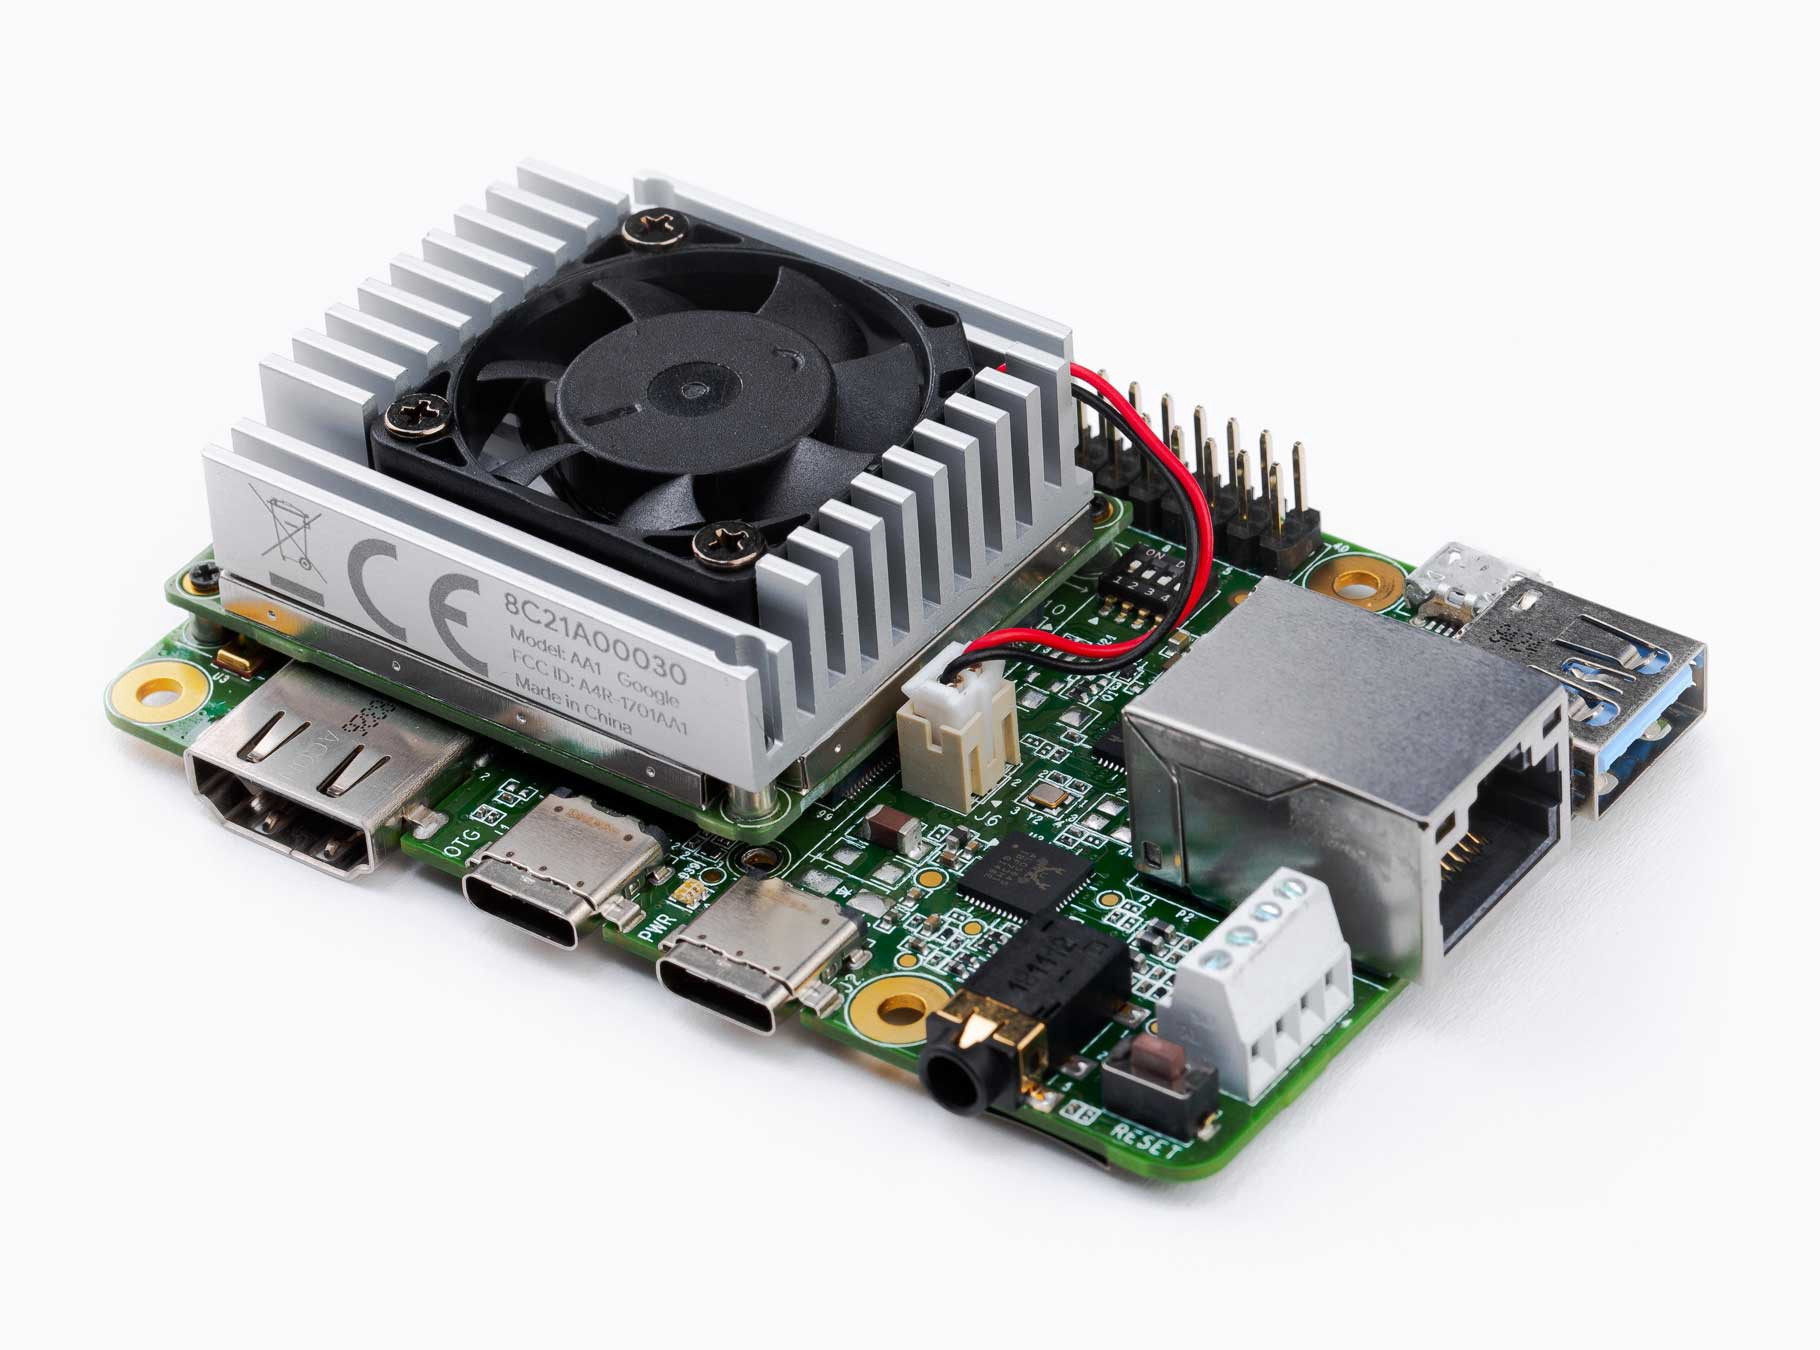
\includegraphics[width=50mm,scale=0.5]{tpu}
	\caption{Some images}\label{fig:foobar}
\end{figure}
\end{frame}

\section{Hardware Comparison CPU vs GPU}
\begin{frame}
	\frametitle{Hardware Comparison CPU vs GPU}
	\subsection{Hardware Comparison CPU vs GPU}
	 \begin{figure}
	 	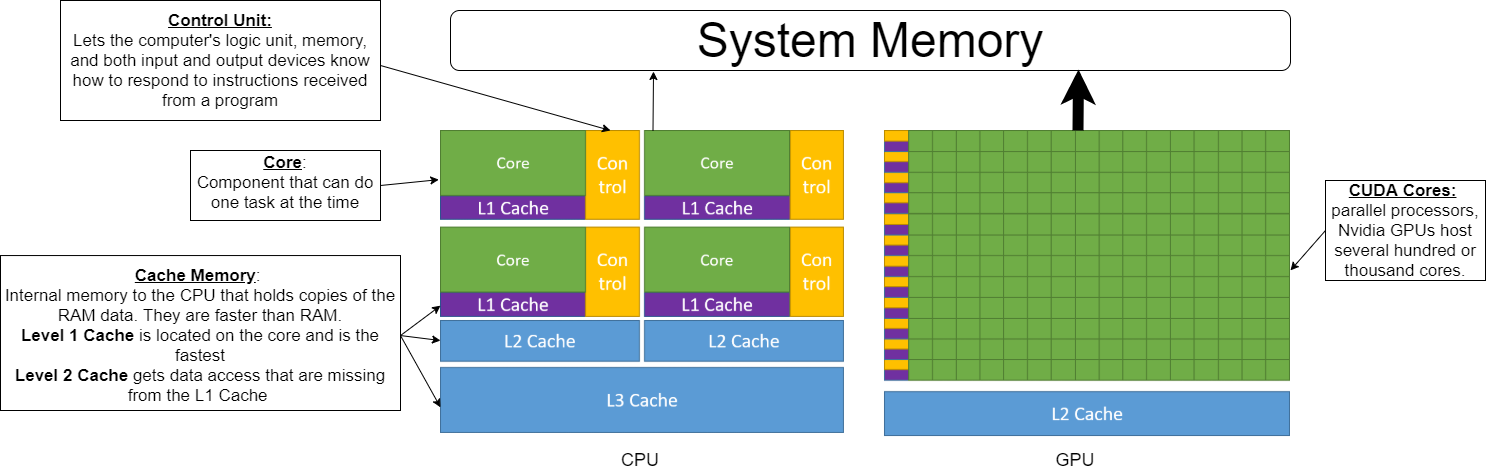
\includegraphics[width=\textwidth,height=\textheight,keepaspectratio]{cpu_vs_gpu}
	 \end{figure}
\end{frame}

\begin{frame}
	\frametitle{Hardware Comparison CPU vs GPU}
\begin{center}
	\begin{tabular}{| c | c | c |}
		\hline
		\textbf{Processor Type} & \textbf{CPU} & \textbf{GPU} \\ 
		\hline
		\textbf{Processor Model} & i9-10900K & Tesla V100 \\  
		\textbf{Manufacturer} & Intel & Nvidia  \\
		\textbf{Processor Speed (Max)} & 5.30 GHz & 1.380 GHz  \\
		\textbf{Memory (up to)} & 128 GB (RAM) & 32 GB (GRAM) \\
		\textbf{Number of Cores} & 10 & 5120 (CUDA cores) \\
		\textbf{Memory Bandwidth} & 45.8 GB/s & 900 GB/s\\
		\textbf{Price} & \textasciitilde R 16 000 & \textasciitilde R 200 000\\
		\hline  
	\end{tabular}
\end{center}
\end{frame}

\section{How does GPU works "faster" than the CPU?}
\begin{frame}
	\frametitle{How does GPU works "faster" than the CPU?}
	\begin{itemize}
		\item \textbf{Larger memory bandwidth}: More data can get in and out the component at a time,
		\item \textbf{Parallelization}: Those many CUDA cores work well in parallel for one given task
		\item \textbf{Fast Memory access}: Multiple L1 and L2 Cache memory,
		\item CUDA API allows you not to worry about memory allocation or deallocation, type of Matrix Multplication to use or how to orchestrate the parallelism of the cores. Some popular frameworks using CUDA:
			 \begin{figure}
			
\includegraphics[width=\textwidth,height=\textheight,keepaspectratio]{dl_frameworks}
		\end{figure}
	\end{itemize}
\end{frame}

\section{Very short demo}
\begin{frame}
	\frametitle{Demo}
	
	We will run short 2 experiments on both the CPU and the GPU:
	\begin{itemize}
		\item Multiplication of 2 scalar: 8.8 x 8.9
		\item Multiplication of 2 relatively big matrices
	\end{itemize}
	
		\centering
	Demo Link: \href{https://colab.research.google.com/drive/1q32stN5vWQ3XApmu58BczJJy62wTI3Zf#scrollTo=UjuLyp2wMK7D}{Colab Experiment}.
\end{frame}

\end{document}